\documentclass{article}
\usepackage{amsmath}
\usepackage{mathtools}
\usepackage{txfonts}
\usepackage{fancyhdr}
\usepackage[margin=0.5in]{geometry}
\usepackage{graphicx}
\graphicspath{ {images/} }

\setlength{\parskip}{\baselineskip}%
\setlength{\parindent}{0pt}%
\pagestyle{fancy}
\fancyhf{}
\renewcommand{\headrulewidth}{0pt}



\begin{document}
\fancyhead[R]{\null\hfill\begin{tabular}[t]{l@{}}
	\textbf{Daniel Hartig} \\
	Stat 652 \\
	Homework 3
\end{tabular}}
\setlength{\headheight}{4\baselineskip}



\subsection*{Problem 1}
\subsubsection*{a.}

\begin{align*}
m_1 = \bar{X} = \mu_1^\prime,\quad\quad \mu_1^\prime &= E\left[\frac{\theta x^{\theta-1}}{3^{\theta}}I_{(0,3)}(x)\right] \\
&=\int_0^3 x\frac{\theta x^{\theta-1}}{3^{\theta}}dx = \frac{\theta}{3^\theta}\int^3_0x^\theta dx \\
&=\frac{\theta}{3^\theta}\left.\frac{x^{\theta+1}}{\theta+1}\right|^3_0 = \frac{3\theta}{\theta+1} \\
\end{align*}
\[\theta = \frac{-\mu_1^\prime}{\mu_1^\prime-3},\quad\quad \hat{\theta}_{MME} = \frac{\bar{X}}{3-\bar{X}}\]

This answer is intuitive because $X_i$ has the range $(0,3)$; therefore $\bar{X}$ must be in this range as well. The denominator must therefore always be a positive number, and the range of $\theta$ becomes $(0,\infty)$, as given in the problem statement.

\subsubsection*{b.}
\begin{align*}
L(\theta|x)&=\prod_{i=1}^n\frac{\theta x_i^{\theta-1}}{3^\theta}I_{(0,3)}(x) \\
\mathcal{L}(\theta|x)&=\sum_{i=1}^n \log{\theta}+(\theta-1)\log{x_i}\,I_{(0,3)}(x)-\theta\log{3} \\
\frac{d\mathcal{L}(\theta|\mathbf{x})}{d\theta} &= \sum_{i=1}^n \frac{1}{\theta} + \log{x_i}\,I_{(0,3)}(x) - \log{3} \\
\end{align*}
Solve for a maximum by setting the derivative of the log-likelihood function equal to zero:
\begin{align*}
\sum_{i=1}^n \frac{1}{\theta} &= -\sum_{i=1}^{n}\log{\frac{x_i}{3}} \\
\frac{n}{\theta} &= -\sum_{i=1}^{n}\log{\frac{x_i}{3}} \\
\hat{\theta}_{MLE} &= \frac{-n}{\sum_{i=1}^{n}\log{\frac{X_i}{3}}}
\end{align*}
Check the second derivative to ensure that this is a global maximum:
\[\frac{d^2\mathcal{L}(\theta|x)}{d\theta^2} = \sum_{i=1}^n -\frac{1}{\theta^2} = -\frac{n}{\theta^2}\]
The second derivative is always negative, so the point in question must be a global maximum. This answer is intuitive, because $x_i<3$; therefore $x_i/3 < 1$; therefore $\log{x_i/3}<0$. The sum of negative numbers is negative in the denominator, while $-n$ is negative in the numerator. Therefore, $\theta$ will be in the range $(0,\infty)$, as given in the problem statement.

\subsection*{Problem 2}
\subsubsection*{a.}
\begin{align*}
m_1 = \bar{X}= \mu_1^\prime,\quad\quad\mu_1^\prime &= E\left[\frac{3x_i^2}{\theta^3}I_{(0,\theta]}(x)\right] \\
&=\int_0^\theta x\frac{3x^2}{\theta^3}dx = \frac{3}{\theta^3}\int^\theta_0x^3dx \\
&=\frac{3}{\theta^3}\left.\frac{x^4}{4}\right|^\theta_0 = \frac{3\theta}{4}
\end{align*}
\[\hat{\theta}_{MME} = \frac{4\bar{X}}{3}\]
\subsubsection*{b.}
\begin{align*}
L(\theta|x) &= \prod_{i=1}^n\frac{3x^2}{\theta^3}I_{(0,\theta]}(x) \\
&=\begin{cases} \frac{3^n}{\theta^{3n}}\prod_{i=1}^n x_i^2 & \theta \geq x_{(n)} \\ 0 & \theta < x_{(n)} \end{cases}
\end{align*}
\[\frac{dL(\theta|x)}{d\theta} = \frac{-n3^{n+1}}{\theta^{3n+1}}\prod_{i=0}^n x_i^2\]
This derivative is always negative, but never reaches zero. Since the derivative is negative, $L$ is always decreasing on $(x_{(n)}, \infty)$. Therefore, the maximum value of the likelihood function is attained when $\hat{\theta}_{MLE} = x_{(n)}$.
\subsubsection*{c.}
\begin{align*}
\int f(x|\theta) &= \int \frac{3x^2}{\theta^3}dx = \frac{x^3}{\theta^3}\\
F(X|\theta)= P(X < x)&= \begin{cases}\frac{x^3}{\theta^3} &x \in (0,\theta] \\ 0 & x \notin (0,\theta]\end{cases}  \\
\end{align*}
The probablility that all of $n$ $X_i$'s are less than $x$ is equal to this expression raised to the $n$ power. Let $Y = X_{(n)}$, then 
\begin{align*}
P(Y < y) &= \frac{y^{3n}}{\theta^{3n}} = F(y|\theta) \\
f(y|\theta) &= \frac{d}{dx}\frac{y^{3n}}{\theta^{3n}} = \frac{3ny^{3n-1}}{\theta^{3n}} \\
E\left[f(y|\theta)\right] &= \int_0^\theta y\frac{3ny^{3n-1}}{\theta^{3n}}dx \\
&= \frac{3n}{3n+1}\left.\frac{y^{3n+1}}{\theta^{3n}}\right|^\theta_0 = \frac{3n}{3n+1}\theta
\end{align*}
As $n$ approaches infinity, $E(\hat{\theta}) = E(X_{(n)}) \to \theta$. 

\subsection*{Problem 3}
\subsubsection{a.}
\begin{align*} 
p_2 \text{  observed} &= \frac{5}{25} = \theta(1-\theta) \\
\theta^2 - \theta +1/5 &= 0 \\
\theta &= \frac{\sqrt{5} \pm 1}{2\sqrt{5}}
\end{align*}
Since $\theta \in (0, 1/2)$, only the lower of the two roots is applicable, so \[\hat{\theta} = 0.276.\]

\subsubsection*{b.}
\begin{align*}
L(\theta|n_1=11, n_2=5, n_3=9) &= \frac{25!}{11!\,5!\,9!} \left(\theta\right)^11\left(\theta(1-\theta)\right)^5\left(\left(1-\theta\right)^2\right)^9 \\
&=C\theta^{16}\left(1-\theta\right)^{23}
\end{align*}
where $C = 25!/(11!\,5!\,9!) = 8923714800$.
\begin{align*}
\mathcal{L}(\theta) &= \log{C} + 16 \log{\theta} + 23 \log{(1-\theta)} \\
\frac{d\mathcal{L}(\theta)}{d\theta} &= \frac{16}{\theta}+\frac{23}{\theta-1}
\end{align*}
Set this derivative equal to zero to solve for maximum:
\begin{align*}
\frac{16}{\theta} &= \frac{23}{1-\theta} \\
\hat{\theta}_{MLE} &= \frac{16}{39} = 0.410
\end{align*}
Check the second derivative to ensure that this is a global maximum:
\[\frac{d^2\mathcal{L}(\theta)}{d\theta^2} = -\frac{16}{\theta^2}-\frac{23}{(\theta-1)^2}\]
Since the second derivative is always negative, $\hat{\theta}_{MLE} = 0.410$ is a global maximum of the likelihood function. 

\subsection*{Problem 4}
\subsubsection*{a.}
\begin{align*}
m_1 = \bar{X},\quad\quad \mu_1^\prime&=\frac{1+\theta x}{2}I_{[-1,1]}(x) \\
&=\frac{1}{2}\int_{-1}^1 x\left(1+\theta x\right)dx \\
&= \frac{1}{2}\left.\left(\frac{x^2}{2}+\frac{\theta}{3}x^3\right)\right|_{-1}^1 = \frac{1}{2}\left(\frac{2\theta}{3}\right) \\
&= \frac{\theta}{3} \\
\hat{\theta}_{MME} &= 3\bar{X}
\end{align*}
\subsubsection*{b.}
\[L(\theta|x) = \frac{1+\theta x_1}{2}\]
The range of both $x$ and $\theta$ are $[-1,1]$. If $x>0$, then likelihood increases with increasing $\theta$, so maximum likelihood is when $\theta =1$. If $x<0$, likelihood decreases with increasing $\theta$, so maximum likelihood is when $\theta = -1$. If $x=0$, likelihood is a constant $1/2$ for all $\theta$. Therefore the maximum likelihood expression is 
\[\theta = \begin{cases}1 & x > 0 \\ [-1,1] & x = 0 \\-1 & x < 0\end{cases}\]
\subsubsection*{c.}
\begin{align*}
L(\theta|x_1=0.5,x_2=-0.1,x_3=0.9,x_4=-0.5) &= \prod_{(i=1}^4 \frac{1+\theta x}{2} \\
&=\frac{1}{16}(1+.5\theta)(1-.1\theta)(1+.9\theta)(1-.5\theta) \\
&=\frac{1}{16}(.0225\theta^4-.2x^3-.34x^2+.8x+1) \\
\frac{dL(\theta)}{dx} &= \frac{1}{16}(.09\theta^3-.6\theta^2-.68\theta+.8) \\
\frac{d^2L(\theta)}{dx^2} &= \frac{1}{16}(.27\theta^2-1.2\theta-.68)
\end{align*}
To use Newton's method to find the roots of the first derivative of the likelihood function, we will need the second derivative. Also, we need an intial estimate. Since $\bar{X}$ is $0.2$, our initial estimate based on the MME is $3(0.2) = 0.6$. I will solve using a Python program written for STAT654, posted here:
\begin{verbatim}
# input function f as a function of x
def f(x):
        return (1/16)*(0.09*x**3-0.6*x**2-0.68*x+0.8)
        
#Derivative of f
def dfdx(x):
        return (1/16)*(0.27*x**2-1.2*x-0.68)
        
# number of iterations
it = 10

# initial guess
x_n = 0.6


# perform iteration
x_n = float(x_n)
for i in range(it):
    x_nplus = x_n - f(x_n)/dfdx(x_n)
    print("Iteration {1}: {4:.2f} = {0:.2f} - {2:.2f}/{3:.2f}".format(x_n,
                                                          i, f(x_n), dfdx(x_n), x_nplus))
    x_n = x_nplus

print("Value of x_n: {0:.5f}".format(x_n))
\end{verbatim}

The result of this execution is:
\begin{verbatim}
Iteration 0: 0.75 = 0.60 - 0.01/-0.08
Iteration 1: 0.74 = 0.75 - -0.00/-0.09
Iteration 2: 0.74 = 0.74 - -0.00/-0.09
Iteration 3: 0.74 = 0.74 - -0.00/-0.09
Iteration 4: 0.74 = 0.74 - 0.00/-0.09
Iteration 5: 0.74 = 0.74 - 0.00/-0.09
Iteration 6: 0.74 = 0.74 - 0.00/-0.09
Iteration 7: 0.74 = 0.74 - 0.00/-0.09
Iteration 8: 0.74 = 0.74 - 0.00/-0.09
Iteration 9: 0.74 = 0.74 - 0.00/-0.09
Value of x_n: 0.74331
\end{verbatim}
We can verify that this is a maxima by looking at the graph of the likelihood function on $[1,1]$:

\begin{center}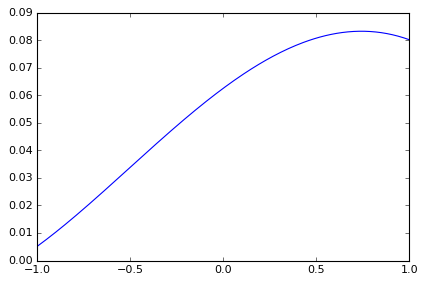
\includegraphics[scale=0.8]{hw3_4_graph}\end{center}

Thus $\hat{\theta}_{MLE}=0.743$ is the maximum within $[-1,1]$. 

\subsection*{Problem 5}
\begin{align*}
m_1 &= \bar{X} = 0.51\bar{66} \\
m_2 &= \frac{1}{n}\sum^n_{i=1}x_i^2 = 1.3113 \\ \\
\mu_i^\prime &= E\left[\frac{1}{2\delta}I_{[\gamma-\delta, \gamma+\delta]}(u)\right] \\ 
&= \int^{\gamma+\delta}_{\gamma-\delta}\frac{1}{2\delta}udu \\
&=\frac{1}{4\delta}\left.u^2\right|^{\gamma+\delta}_{\gamma-\delta} = \frac{1}{4\delta}\left(4\gamma\delta\right)\\
& = \gamma \\ \\
\mu_2^\prime &= E\left[\left(\frac{1}{2\delta}\right)^2 I_{[\gamma-\delta, \gamma+\delta]}(u)\right] \\
&= \int^{\gamma+\delta}_{\gamma-\delta}\frac{1}{4\delta^2}udu \\
&= \frac{1}{8\delta^2}\left(4\gamma\delta\right) \\
&= \frac{\gamma}{2\delta}
\end{align*}
\begin{align*}
\hat{\gamma}_{MLE} & = m_1 = 0.517 \\
\hat{\delta}_{MLE} & = \frac{\gamma}{2m_2} = \frac{0.51\bar{66}}{2\cdot1.3113} = 0.197
\end{align*}



\end{document}